\chapter{Results}\label{ch:results}
In this chapter I show how the pruning with heuristic affects MobileNet
v1\cite{howard2017mobilenets} based models. The experiments will be run using
both CIFAR-10\cite{cifar_10} and ImageNet 2012\cite{imagenet_cvpr09}.
Before showing to the results, I'll give an overview about MobileNet v1
architecture and the respective datasets used in the experiments.

\section{MobileNet v1}
MobileNet is a class of efficient models for mobile and embedded vision
applications (\autoref{fig:mobilenet_applications}) developed by Google.
It is based on a streamlined architecture that uses depthwise separable
convolutions to build light weight deep neural networks.

\begin{figure}[ht]
    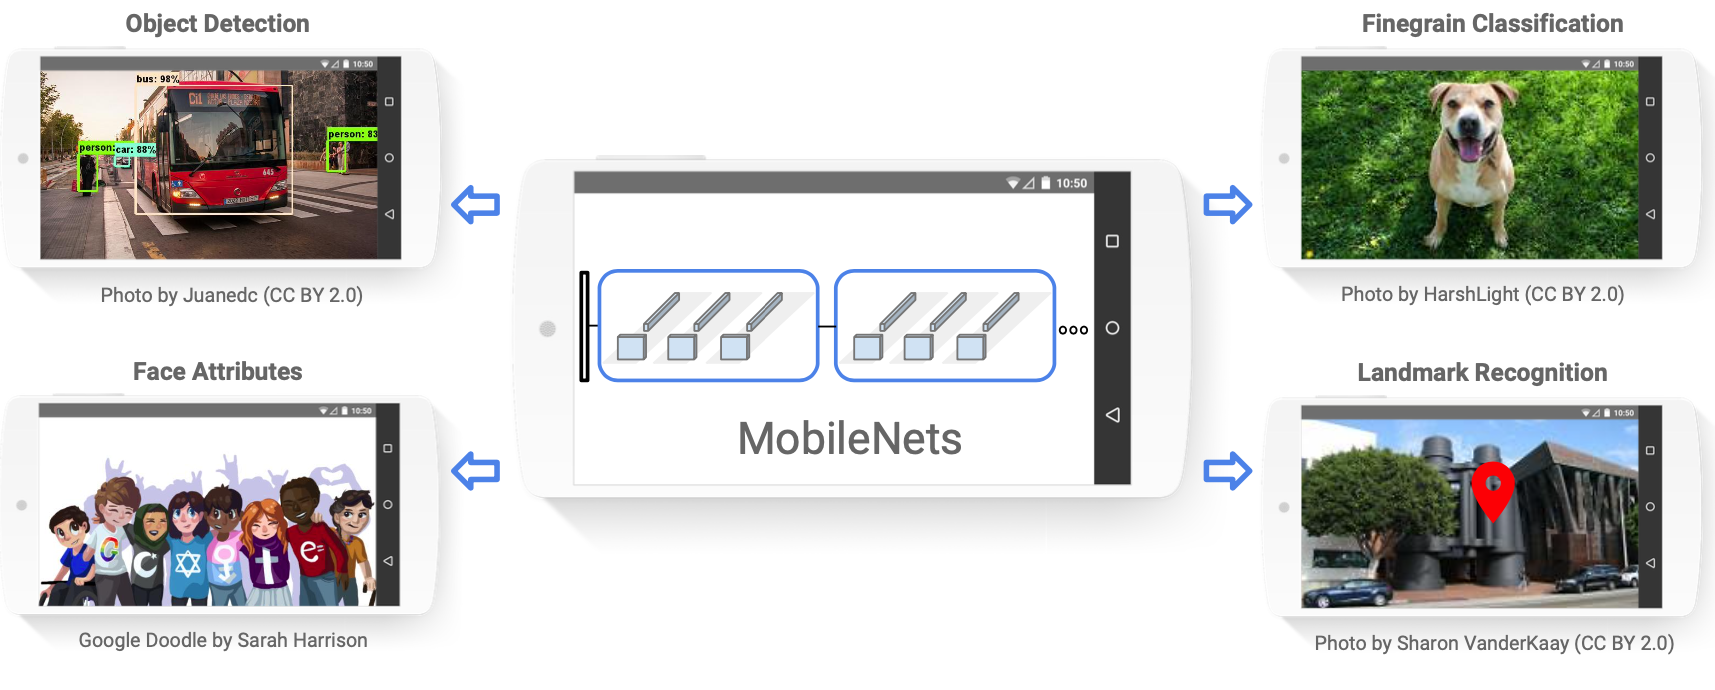
\includegraphics[width=\textwidth]{images/results/mobilenet_applications.png}
    \centering
    \caption{MobileNet applications}\label{fig:mobilenet_applications}
\end{figure}

Convolutional neural networks have been more popular in the recent years and
their accuracy increased thanks to more complex architecture increasing their
size whilst impacting negatively in speed. In many real world applications,
these networks need to run on edge devices with limited resources and the
inferences need to be carried out in a timely fashion.

The main focus of MobileNet is to increase the efficiency of the network by
decreasing the number of parameters by not compromising
performance\cite{review_mobilenet}.

\subsection{Depthwise Separable Convolution}
Depthwise separable convolution is the core basis of MobileNet architecture. It
is a \textbf{depthwise convolution followed by a pointwise convolution}.

A normal convolution is shown in \autoref{fig:convolution}

\begin{figure}[ht]
    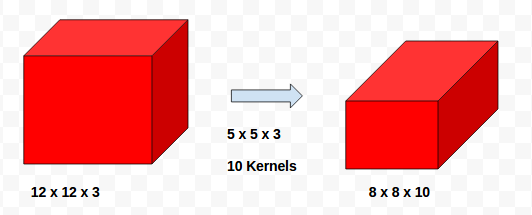
\includegraphics[width=10cm]{images/results/convolution.png}
    \centering
    \caption{Convolution}\label{fig:convolution}
\end{figure}

In the figure there is an input image size of $12\times12\times3$ and the
kernel (or filter) is $5\times5\times3$ with stride = 1. There are though 10
kernels to apply and this gives an output image of $8\times8\times10$.
The total computational cost is \bm{$12\times12\times5\times5\times3\times10 =
108000$}.

There are the following dimensions:
\begin{itemize}
    \item Input image: \bm{$D_f \times D_f \times M$}
    \item Output image: \bm{$D_f \times D_f \times N$}
    \item Convolution kernel: \bm{$D_k \times D_k \times M \times N$}
\end{itemize}

So in a normal convolution the total computational cost is
\bm{$D_k \times D_k \times M \times N \times D_f \times D_f$}

The above convolution can be split in 2 phases:
\begin{enumerate}
    \item Depthwise convolution
    \item Pointwise convolution
\end{enumerate}

The first one is the \textbf{depthwise convolution} and it is shown in
\autoref{fig:depthwise_convolution}.

\begin{figure}[ht]
    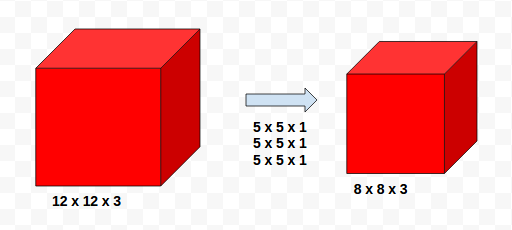
\includegraphics[width=10cm]{images/results/depthwise_convolution.png}
    \centering
    \caption{Depthwise convolution}\label{fig:depthwise_convolution}
\end{figure}

In this case the input has 3 channels and there are 3 $5\times5\times1$
kernels. These 3 kernels are applied to the three channels respectively
producing 3 $8\times8\times1$ output. When the 3 outputs are stacked the final
output is $8\times8\times3$.

The second phase is the \textbf{pointwise convolution} as shown in
\autoref{fig:pointwise_convolution}.

\begin{figure}[ht]
    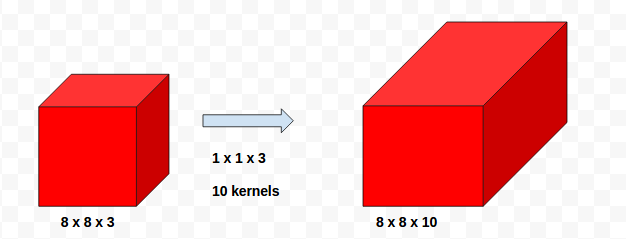
\includegraphics[width=10cm]{images/results/pointwise_convolution.png}
    \centering
    \caption{Pointwise convolution}\label{fig:pointwise_convolution}
\end{figure}

The output image of the previous step is the input image for this step.
The convolution is done using a $1\times1\times3$ kernel on the input image
producing a feature map. Repeating this using 10 different $1\times1\times3$
kernels will produce 10 different feature maps that will be stacked together.

The computation for each step is:
\begin{enumerate}
    \item Depthwise convolution: \bm{$12 \times 12 \times 5 \times 5 \times 3 =
        10800$}
    \item Pointwise convolution: \bm{$8 \times 8 \times 3 \times 10 = 1920$}
\end{enumerate}

Therefore the total number of computations is \textbf{10800 + 1920 = 12720}

More generically the computational cost is \bm{$D_k \times D_k \times M \times
D_f \times D_f + M \times N \times D_f \times D_f$}

In this specific case using a kernel of $3 \times 3$ there is about 8 to 9
times less computational reduction: \bm{$108000 / 12720 \approx 8.45$}

\subsection{MobileNet architecture}
The network architecture is built on depthwise separable convolutions except
for the first layer which is a full convolution

There are 28 convolutional layers (counting depthwise and pointwise layers) and
1 fully connected layer followed by a softmax layer
(\autoref{fig:mobilenet_architecture}).

\begin{figure}[ht]
    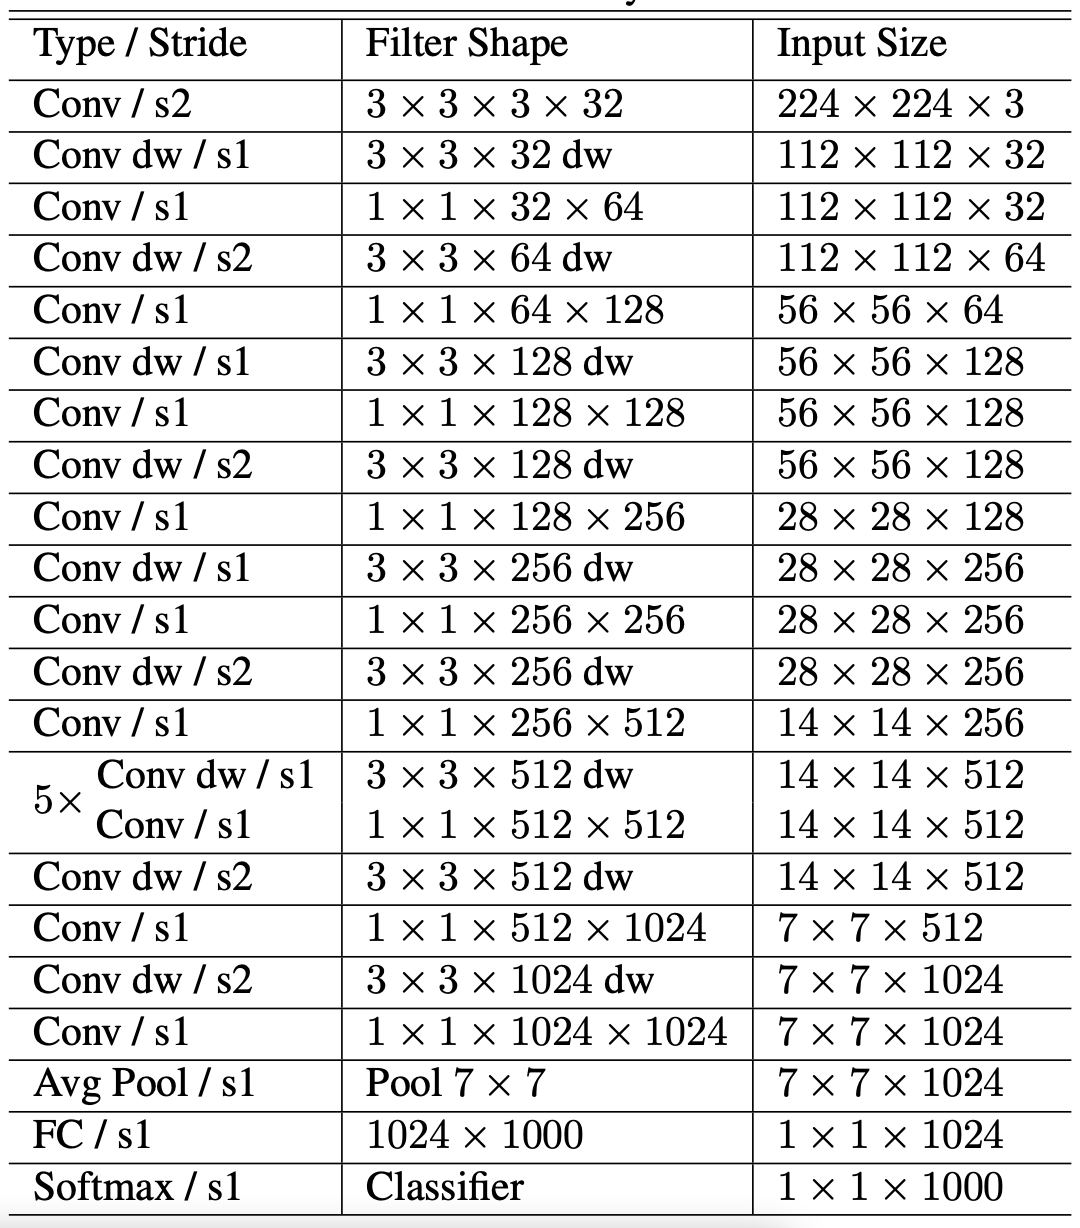
\includegraphics[width=10cm]{images/results/mobilenet_architecture.png}
    \centering
    \caption{MobileNet architecture}\label{fig:mobilenet_architecture}
\end{figure}

All layers are followed by a batch normalization and ReLU non linearity
(\autoref{fig:mobilenet_convolution}) with the exception of the final fully
connected layer which has no non linearity and feeds into a softmax layer for
classification.
As seen earlier in the thesis, the softmax is used to to predict a single class
of K mutually exclusive classes. In the case of MobileNet, when used with
ImageNet, it can classify up to 1000 classes.

\begin{figure}[ht]
    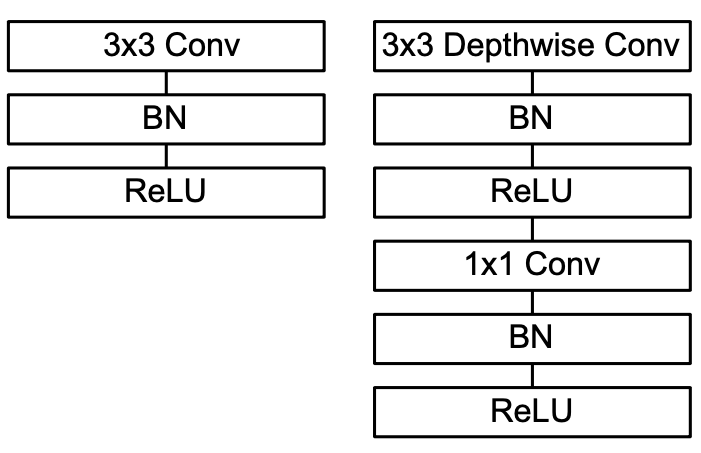
\includegraphics[width=8cm]{images/results/mobilenet_convolution.png}
    \centering
    \caption{Normal convolution vs MobileNet convolution}\label{fig:mobilenet_convolution}
\end{figure}

\subsection{Width Multiplier}
MobileNet has been developed to be small and low latency but sometimes specific
use cases or applications need the model to be faster and smaller.
In order to construct these smaller and less computationally expensive models
a very simple parameter \bm{$\alpha$} called width multiplier has been
introduced.

The role of the width multiplier $\alpha$ is to thin a network uniformly at
each layer: the number of input channels M becomes $\alpha M$ and the number of
output channels N becomes $\alpha N$.

So depth wise separable computational cost becomes \bm{$D_k \times D_k \times
\alpha M \times D_f \times D_f + \alpha M \times \alpha N \times D_f \times
D_f$} where $\alpha \in \interval[open left]{0}{1}$ with typical settings of 1,
0.75, 0.5, 0.25.

The \autoref{fig:mobilenet_widthmultiplier} shows the impact that $\alpha$ has
on accuracy, numbers of operations and parameters.

\begin{figure}[ht]
    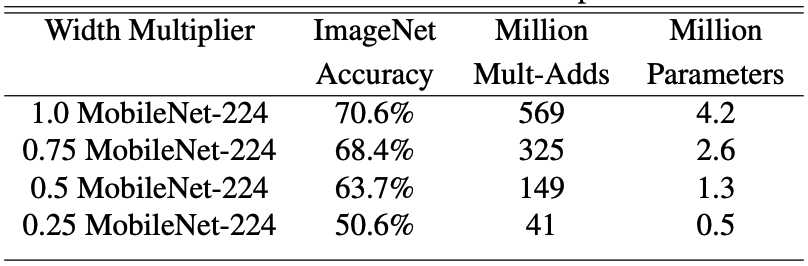
\includegraphics[width=10cm]{images/results/mobilenet_widthmultiplier.png}
    \centering
    \caption{Width multiplier impact}\label{fig:mobilenet_widthmultiplier}
\end{figure}

In this thesis I consider \bm{$\alpha = 1$} to be the baseline.

\subsection{Resolution Multiplier}
The second hyper-parameter to reduce the computational cost of a neural network
is a resolution multiplier \bm{$\rho$}. This can be applied to the input image
and the internal representation of every layer is subsequently reduced by the
same multiplier.
Including $\rho$, the computational cost becomes \bm{$D_k \times D_k \times
\alpha M \times \rho D_f \times \rho D_f + \alpha M \times \alpha N \times \rho
D_f \times \rho D_f$} where $\rho \in \interval[open left]{0}{1}$i which is
typically set implicitly so that the input resolution of the network is 224,
192, 160 or 128.

The \autoref{fig:mobilenet_resolutionmultiplier} shows the impact that $\rho$
has on accuracy, numbers of operations and parameters.

\begin{figure}[ht]
    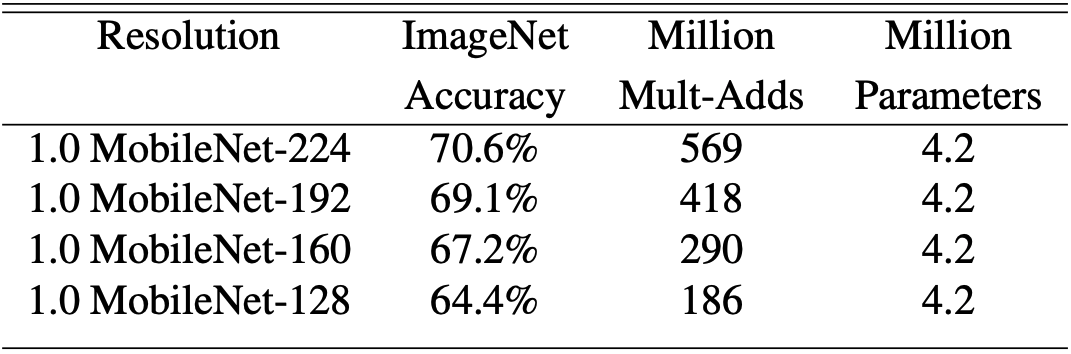
\includegraphics[width=10cm]{images/results/mobilenet_resolutionmultiplier.png}
    \centering
    \caption{Resolution multiplier impact}\label{fig:mobilenet_resolutionmultiplier}
\end{figure}

In this thesis I consider \bm{$\rho = 1$} to be the baseline.

\section{Result with MobileNet v1 and CIFAR-10}
\lipsum[1]

\subsection{CIFAR-10 dataset}
\lipsum[1]

\subsection{Experiment results}
\lipsum[1]

\section{Result with MobileNet v1 and ImageNet 2012}
\lipsum[1]

\subsection{ImageNet 2012 dataset}
\lipsum[1]

\subsection{Experiment results}
\lipsum[1]
